\section{Design Decisions}
	Before starting the actual implementation of the desired tool, it was necessary to make some fundamental design decisions regarding the work at hand such as
	\begin{itemize}
	\item required features,
	\item used code base,
	\item included external libraries and tools,
	\item applied programming and description languages,
	\item ways of directing the users workflow, and
	\item increasing the applications usability by appropriate visualization techniques.
	\end{itemize}
	
	Some of the choices made had to be revised during the implementation process and additional design cornerstones were added when required to achieve certain goals. 
	
%TODO github
%TODO open source	
	
\subsection{Choice of Language, Libraries and Frameworks}
	\label{sec-languages-frameworks}
	
	\paragraph{Research of Integration Possibilities into Existing Tools}
		The initial idea was to integrate the use-case proposed by the problem statement into an existing tool.
		\Gls{qucs}\cite{Qucs:base} seemed to be an obvious choice for that purpose due to its already existing visual design capabilities, availability of source code and sufficiently large community of users and contributors.
	% Code quality and documentation / time consuming
		When researching ways to integrate the requested features however, it was found that the code quality was low and documentation was largely missing.
	% ongoing restructuring
		The developers were aware of these shortcomings, and at the time of writing, \gls{qucs} is subject to an extensive refactoring process.
	
		Some attempts were made to extend the code base, allowing the extraction of the internal model in a netlist format for further processing by other tools. 
	% Components hard-coded
		The components used in the schematic turned out to be hard-coded into the tool.
		Due to the points mentioned above, it quickly turned out to be a time-consuming, difficult and error-prone effort to achieve even minor results.
	% Ergo: not qucs
		This situation led to the decision not to expand \gls{qucs} as proposed by the initial task.
		Research for other tools that could be used for integrating the desired functionality did not reveal any alternatives that were deemed viable.
		Developing a new tool for the intended use case therefore was regarded as the best way to proceed.
		
	\paragraph{Used Languages and Frameworks}		
	% C++11 and Qt
		The experiences made earlier 
		when investigating \gls{qucs} yielded the insight that it would be a good choice to use a combination of a well-established high-level language in combination with a framework that could provide powerful tools and abstractions to reduce the effort needed to implement the \gls{ui}.\footnote{
			Experience shows that \gls{ui} implementations, especially for graphical ones,  consist of huge portions of configuration code that can be generated automatically. 
			It is a noticeable relief for the developer to do so.
			\cite{UIgen} \cite{UIgen2}
		}
		
		A suitable combination was found in using the \emph{C++} programming language together with the \gls{qt}-framework.
	% choice of C++11
		While the \emph{C++14} standard was not yet commonly supported by development tools at the time of writing, \emph{C++11} had been well established and offered features that were found desirable for the task at hand.
		Due to the large set of features offered by \gls{qt}, it turned out not to be necessary to include further frameworks to achieve the intended results.
		As a consequence, the major part of the \gls{ui} is described using the \gls{xml}.

	% Json for user-based definitions and persistence
		It was aimed at using a very simple, human-readable format to allow the user easy access to the stored data for modification and debugging purposes.
		Therefore, \Gls{json} has been employed to represent user-defined components and data persistence.
		Since it is easy to parse by a program\footnote{
			\gls{qt} already offers means of writing and parsing \gls{json}, which simplifies the implementation considerably.
		} and can also be fairly well edited by a human user with a simple text editor, this format proved to be a good choice during implementation.
		This will also become an important aspect in section \ref{sec-basic-interaction} and \ref{sec-user-defined-components}.

\subsection{Solving the QBF Problem}
	\label{sec-solving-qbf}
		
	In section \ref{sec-theoretical-background}, it was established that solving \gls{qbf} is one way to compute a configuration in order to be able to evaluate whether a given target function can be implemented by a provided circuit design.
	Applying a dedicated \gls{qbf} solver instead of transforming the problem into \gls{sat} first has some clear advantages:

	\begin{itemize}
		\item It eliminates the need for intermediate representations and expansion logic between \gls{qbf} and \gls{sat} representations.\footnote{
			A \gls{qbf} problem's size will grow exponentially, when transformed into \gls{sat} as noted in section \ref{sec-qbf-to-sat}.
		}
		\item Established \gls{qbf} solvers are very well optimized and, therefore, perform much better than any implementation of non-specialized programmers can be  reasonably expected to do.
	\end{itemize}
	
	An extensive comparison of currently available \gls{qbf} solvers was composed by \textsc{Narizzano et\,al.} \cite{qbfComparison}.	
		
	From this, \gls{quantor} was selected as backing tool for this task, providing the capabilities mentioned above.

	In contrast to most other tools, it not only decides whether a problem is satisfiable, but also yields a variable assignment for the outermost existential quantor, if there is any.
	It thus computes the desired configurations.
	
	\Gls{quantor} is provided as source code and can be easily included either by directly compiling it into the application by or generating a linkable library.
		
	\paragraph{Interfacing Quantor}
		The input to \gls{quantor} has to be provided in \gls{cnf}. 
		So it is necessary to create an interface that transforms the formulae specifying the internal model and target formulae in an appropriate way for the \gls{qbf} solver to use and interpret the returned results to obtain a conclusive solution that can be presented to the user.
		For doing so, the computed result must be interpreted and prepared for visual representation.
		The concrete implementation of the classes responsible for this step can found in section \ref{sec-quantor-interface}. 
		
		
\subsection{Design of the Internally Used Meta-Model}
	\label{sec-model-design}	
	
	While researching how \gls{qucs} handled components, it was discovered that the wide variety of available building blocks used for circuit design were directly included as classes in the source code.
	This might be a sound decision for the tool in question but it also was evident that thereby the maintainability and introduction of new components was notably inhibited.
	From the experiences made arose the desire to use a different approach in \emph{q2d}. 
			
	A \emph{component meta-model} has been designed to represent and categorize a hierarchy of templates, from which the actual building blocks for the actual model can be derived.
	 
	\paragraph{Abstraction into Component Types}
		When designing schematics, it becomes obvious very quickly that most components do have a lot of things in common and share structural and behavioural similarities.
		Commonly used \glspl{hdl} handle this by introducing types or type-like semantics of which a component can be.
		This approach was adopted in \emph{q2d} by introducing a meta-model which describes a hierarchy of component categories and component types.
		From the latter, concrete component instances can be created.
		Categories, on the other hand, are intended mainly for helping with keeping an overview, even if a lot of component types are present.
		In the following the term \emph{component library} will be used as a generalization of any category containing component types.
		Further, component libraries are not restrained from containing sub-libraries, unless explicitly stated otherwise in the context.
	
	\paragraph{Allowing User-Defined Component Types}
		No matter how many pre-defined component types are delivered with the application, users will most likely find that some component they need for their design is missing.
		Since most hardware producers maintain their own catalogues of components, which are updated frequently, it is not feasible to keep the application up-to-date on a regular basis.
		Especially, if components were hard-coded into the application, any changes to the component libraries would require a rebuild of the whole application and a new release.
		As a result, it was deemed far more practical if users were allowed and enabled to create their own components and component libraries.
		To do so, each component type is specified by a \emph{component descriptor file}, which itself is only a simple \gls{json} file following a defined structure.
		This will be discussed in depth in section \ref{sec-user-defined-components}.
		
\subsection{User Interface Ergonomics}
	\label{sec-ui-ergonomics}
	
	The way a user interface is designed has a strong influence on how the user approaches the task they wish to accomplish.
	As a consequence, the \gls{ui} should, amongst other things: 

	\begin{itemize}
		\item Offer sufficient tools to solve the given task while avoiding to become overburdened with features that have little to no use or can be reasonably achieved otherwise.
			The latter often increases the complexity of a program noticeably while offering little value in return. 
		\item Follow semantics that the user can anticipate and comprehend. 
			Preferably, these do require little to no explanation and feel intuitive.
		\item Attempt to discourage creations by the user that might be regarded as flawed or undesirable.
	\end{itemize}		
	In the following, examples for design decisions regarding these points are given.\footnote{
		It would exceed the extend of this document to elaborate all of the design decisions that were made before and during the implementation in detail.
	}
	 
	\paragraph{Disallow Connecting Output Ports to Each Other}
	% disallow connecting output ports
		When designing circuits, it is technically possible to connect multiple output ports of one or several components to the same input port, as shown in figure \ref{fig-connected-outports}. 
		This design method is often used to increase the driving strength of output signals.	
		This practise tends to lead to problems in the resulting circuit, should the output ports assume different signal levels at the same time. 
		In the worst case, the physical implementation might be damaged.
		For this reason, it was decided to disallow the driving of an input port by multiple sources and to have a connecting element to be connected to at most one output port.\footnote{
			An alternative approach would be to introduce formal verification to ensure all drivers always carry the same signals at the same time.
			Any solution output by \gls{quantor} would ensure the outputs carry the same signals in a static state.
			However, timing behaviour has to be considered, which would make this approach become very complex quickly and create the need for a lot of very specific details like timing behaviour of the actual components used in the physical implementation.
			Any formal verification could only be made for a specific setup and had to be re-evaluated whenever the circuit design changes.
		} 
		This is achieved by only allowing to start drawing a wire via dragging forth from an output port and only end this procedure by either dropping over an input port to create a connection or by dropping it on a blank area, thus cancelling the process.
	
	\paragraph{Draw Connections Only in Signal Flow Direction}
		As a consequence of the restrictions mentioned above, the user is forced to always draw connections between components according to the signal flow direction.
		It was theorized, while testing the application, that this restriction might force the user to plan his designs ahead in more detail and reduce the likelihood of design errors.
		A separate study would be required to measure these effects though.
	
	\paragraph{Disallow Mixed-Direction Ports}
		In the early stages of the application design, it was considered to not only support \emph{input} and \emph{output} ports in components but also a variant that could change its direction, similar to \emph{inout} ports known from most \glspl{hdl}.
		This would contradict the decisions made before and noticeably complicate the implementation, especially with respect to the interface of the \gls{qbf} solver.
		Since those mixed-direction ports can be safely emulated by using a separate port for each direction, it was judged to explicitly support only single-direction ports.
		Also, it has to be noted, that it is highly unusual for \glspl{clb} to be produced with mixed-direction ports.
	 %TODO show the replacement as figure 

\subsection{Aspects of Schematic Visualization}
	\label{sec-visualization-aspects}
	Humans are very focused on optical perception of information, which naturally puts an emphasis on the way things are represented visually and can be interacted with.
	Implementing appropriate means of aiding the user perceiving important information faster turned out to be very work-intensive. 
	While a huge amount of visualization techniques exists,
	only a subset could be considered for the actual implementation\cite{InteraktiveSysteme}. 
	
	\paragraph{Aiding Orientation on Larger Schematics}
		As soon as a schematic contains more than a handful of components and connections, it becomes notably harder to maintain the overview and the available screen space might no longer suffice to display everything at once.
		The most common solution for this problem is to add scrolling capabilities to the view area.
		Since the scrolling elements on their own require space on the view as well, it was concluded that a \emph{scrolling on demand} approach posed a good compromise.
	%dot grid to aid orientation
		To further aid the user's orientation on the view area and helping with the alignment of the schematics elements, a dot grid was added.
		It was found to be a better alternative to a line-based grid, which was perceived as more distracting and creating the illusion of a slightly darkened background.
	
	\paragraph{Providing Details on Demand}
		Attempting to provide all available information at once tends to clutter visual representations rather quickly.
		A set of so called \emph{details on demand}-techniques is available to counter information overload.
		In the application at hand, tool tips are employed to obtain information about certain elements.
		If this is not sufficient to display all available details, double-clicking an element will yield all information in a separate window.
		Furthermore, connections will highlight when hovered over so that it is easier for the user to see which elements they are linking.
	
	\paragraph{Visual Representation of Ports}
		Ports are associated with information regarding their signal flow direction, the elements, between which they are interfacing, and their connection status.
		In the first versions of the application, ports were displayed as circles with a filling color depending on their signal flow direction with respect to their owning component.
		However, this led to confusion as they tended to be mistaken for negations.
		While in hand-drawn schematics, simple forms dominate since they can be produced quickly and easily, on computer-generated views, it is feasible to employ more complex shapes, which have the potential to change depending on their state and thus can convey more information.
		It was therefore decided to enhance the representation of ports following a semantic of \emph{adapters and adaptees}.
	
		An \emph{adapter} is a port that receives a connection, which is usually the case for input ports.
		\emph{Adaptees}, on the other hand, provide a signal, which can be received by its counterpart.
		Both elements are displayed in figure \ref{fig-port-semantics}.
		Additionally, when connecting ports, the endpoints of the connection will complement the existing port symbols with their counterparts to create the visual impression of a plug connection.
		These semantics go well with the restrictions of connection drawing discussed in section \ref{sec-ui-ergonomics}.
	%visual representation, no circular shape, no triangle shape
		Regarding the basic shape of these elements, circular forms, looking similar to the \emph{lollipop}-shapes known from \gls{uml} were discussed and rejected as still looking to similar to negations.
		For the same reason triangular versions were discarded\footnote{
			They looked too close to the \gls{din}-symbols for ports with polarity indicators for negated logic, as well as clock driven ports.
		}, and shapes based on squares were chosen.
		The color scheme devised in earlier versions has been kept, assigning a green color to input ports and using red for output ports.
		A slightly grey \emph{active region} surrounds the port symbols to give the user a hint that special interaction options, like drawing connections, are available.
		Symbols of ports that are already connected are set to be more transparent, thus reducing the amount of dominant visual elements and helping the user find ports that are still unconnected.
		The actual representation as implemented is shown in figure \ref{fig-ports-actual}.

	\paragraph{Module Interfaces}
	To aid the understanding of the following sections, the concept of a \emph{module interface} will be introduced briefly.
	A whole circuit, as contained in a single document is synonymously called a \emph{module}.
	Special elements that act as an interfacing point between the module and the outside world are consequently named \emph{module interfaces}.
	If such a module interface conveys data from the outside world into the circuit, it may be considered an \emph{input}.
	When viewed from the inside of the module however, an input appears to emit data.
	\emph{Outputs} behave exactly the other way around.
	This matter is solved by implementing module input and output interfaces conceptually comparable to components, with an actual module port as child element.
	%TODO figure input port
	%TODO figure output port
	When talking about ports, usually the context makes clear, which kind of port is referred to or it will be explicitly stated. 	

	% --- Figures ---
	\begin{figure}
		\centering
		\begin{subfigure}{0.3\textwidth}
		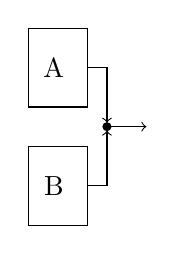
\begin{tikzpicture}
\draw[->] (0, 1.25) rectangle (0.75, 0.25);
\draw (0.325, 0.75) node {A};
 
\draw (0, -0.25) rectangle (0.75, -1.25);
\draw (0.325, -0.75) node {B};

\draw[->] (0.75, 0.75)  -- (1, 0.75) -- (1, 0.05);
\draw[->] (0.75, -0.75) -- (1, -0.75) -- (1, -0.05);

\filldraw (1, 0) circle (0.05);

\draw[->] (1, 0) -- (1.5,  0);
\end{tikzpicture} 
		\caption{Two components \emph{A} and \emph{B} with connected output ports}
		\small{Arrows indicate signal flow direction.}
		\label{fig-connected-outports}
	\end{subfigure}
	\quad
	\begin{subfigure}{0.5\textwidth}
		\centering
		\input{diagrams/port_semantics}
		\caption{The elements of port semantics visualized}	
		\label{fig-port-semantics}
	\end{subfigure}
	
	\begin{subfigure}{0.9\textwidth}
		\centering
		\input{diagrams/ports_actual_look}
		\caption{Actual presentation of connected and unconnected ports}
		\label{fig-ports-actual}
	\end{subfigure}
	
	\caption{Port and Signal Flow Visualization}
	\end{figure}
		
\subsection{Limitations}
	\label{sec-implementations-limitation}
	
	With a wide range of techniques for visualization available and many potential uses for the models that result from the visual design of circuits, it is also important to decide upon limitations of the applications implementation.
	
	\paragraph{Usability Restrictions}
	% zooming, component rotation, active-edge scrolling, snapping
		Features like zooming, rotation of schematic elements, cursor snapping to the dot grid and active-edge scrolling, were considered, but rejected as their estimated implementation effort did not meet with the projected gains in usability, especially with respect to the time limit imposed by the assignment.\footnote{
		The author is also aware that the tool often implies in the visualization that the data flow is oriented from left to right, which is not agnostic to the users culture.
		Later versions of the tool are intended to drop this restriction.
		}
	
	\paragraph{Functional Constraints}
	% no components with state
	% no simulation (for now)
		Even though a feasible extension of the model at hand, the implementation of state was not pursued.
		As a result, it is not possible to simulate any behaviour, and the use of state-bearing components like \emph{flipflops} is not allowed. 